%=======================================================================
% Virtual BMS co-verification whitepaper
% Build: ~/.local/bin/tectonic whitepaper.tex
%=======================================================================
\documentclass[11pt]{article}

\usepackage[margin=1in]{geometry}
\usepackage[T1]{fontenc}
\usepackage{microtype}
\usepackage{booktabs}
\usepackage{tikz}
\usetikzlibrary{arrows.meta,positioning,calc,fit}
\usepackage[europeanresistors]{circuitikz}
\usepackage{caption}
\usepackage[hidelinks]{hyperref}

\newcommand{\iic}{I\textsuperscript{2}C}
\newcommand{\reg}[1]{\texttt{#1}}

\tikzset{
  blk/.style  ={draw, rounded corners=2pt, align=center, inner sep=6pt,
                minimum height=9mm, font=\small},
  hot/.style  ={blk, thick, draw=blue!60!black, fill=blue!60!black!8},
  lbl/.style  ={font=\footnotesize, text=black!60},
  arr/.style  ={-{Stealth[length=2.2mm]}, semithick},
  arrh/.style ={arr, blue!60!black},
}

\title{\bfseries Co-Verifying BMS Firmware Against a Virtual Board:\\
       SV-RNM, a Behavioural BQ76952-Class AFE, and UVM-MS}
\author{Vrajesh Prakhya}
\date{October 2, 2026}

\begin{document}
\maketitle

\begin{abstract}
\noindent
We verify unmodified battery-management host firmware against a fully
virtual six-cell battery board: no silicon, no lab bench.  The
board's analog electronics are SystemVerilog real-number models
(SV-RNM), the battery-monitor AFE is a behavioural model of a
BQ76952-class device with its own register map and hardware protection
engine, and the host firmware (C, stepped cycle-by-cycle through DPI)
talks to it over a pin-level, open-drain \iic{} bus.  A UVM-MS
environment (the randomized-stimulus-and-checking testbench layer
from the silicon-verification world) sits above the board,
pushes physical scenarios at it (cell voltages, load current,
temperature, component tolerances) and checks both what the firmware
reports and what the analog domain actually does.  A 13-scenario regression passes with zero failures on
the xezim simulator, covering measurement accuracy, all four
protection regions, cell balancing, EMI on the shunt sense line, and a
full trip-and-recover sequence.  During bring-up the bench caught
three real defects before any hardware existed, including a one-bit
protocol error that silently broke every bus transaction.

The firmware is verified on both of a firmware team's first two
test rungs, each with the analog board on the other side instead of
a mock: the host-compiled logic, graded by the testbench across the
13-scenario randomized regression above, and then, recompiled as
bare-metal ARM code, the binary itself, booted
on an emulated STM32 under unmodified mainline QEMU, driving the
SV-RNM board over a lockstep socket bridge and reporting the full
trip-and-recover mission over its own UART, with a board timeline
that is reproducible to the nanosecond.  A fault-injection
campaign closes the loop on trust: one deliberate defect per layer
(firmware configuration, firmware protocol, analog front-end, pin
path), each caught by a different rule of a cross-domain checker,
with the clean setup still green.
\end{abstract}

%=======================================================================
\section{The problem: bugs that live between firmware and analog}
%=======================================================================

A battery management system fails in the seam between two worlds.  The
firmware can be unit-tested against mocked register values, and the
digital logic can be simulated, but neither catches the class of bug
where correct-looking code meets real electrical behaviour: a
protection threshold written to the wrong register, a reading that
silently scales wrong at a supply corner, a balancing command that
measures differently than it acts, or a trip that toggles a GPIO while
the actual current keeps flowing.

These bugs normally surface on the lab bench, late, one board spin in.
Firmware mocks cannot find them, because the mock returns whatever the
test author \emph{believed} the analog chain does.  Digital-only
simulation cannot find them, because the interesting behaviour (IR
sag, sensor tolerance, saturation, EMI) is analog and lives on the
PCB, outside the chip.

The approach demonstrated here closes that seam in simulation:
\begin{enumerate}
  \item model the board's analog chain as SV-RNM \emph{functional
        blocks} (not per-passive netlists),
  \item run the actual firmware against it through the real bus
        protocol it would use on hardware, and
  \item put a UVM-MS testbench above both, so physical corners and
        firmware responses are exercised and checked together, with
        functional coverage over their cross product.
\end{enumerate}

%=======================================================================
\section{System under test}
%=======================================================================

The demonstrator mirrors a production BMS architecture (cf.\ the open
6S-BMS project, STM32G0B1 + BQ76952): the measurement and protection
intelligence sits in a dedicated battery-monitor AFE, and a host MCU
supervises it over \iic{}.  Figure~\ref{fig:arch} shows the five
pieces and how they connect.

\begin{figure}[htbp]
\centering
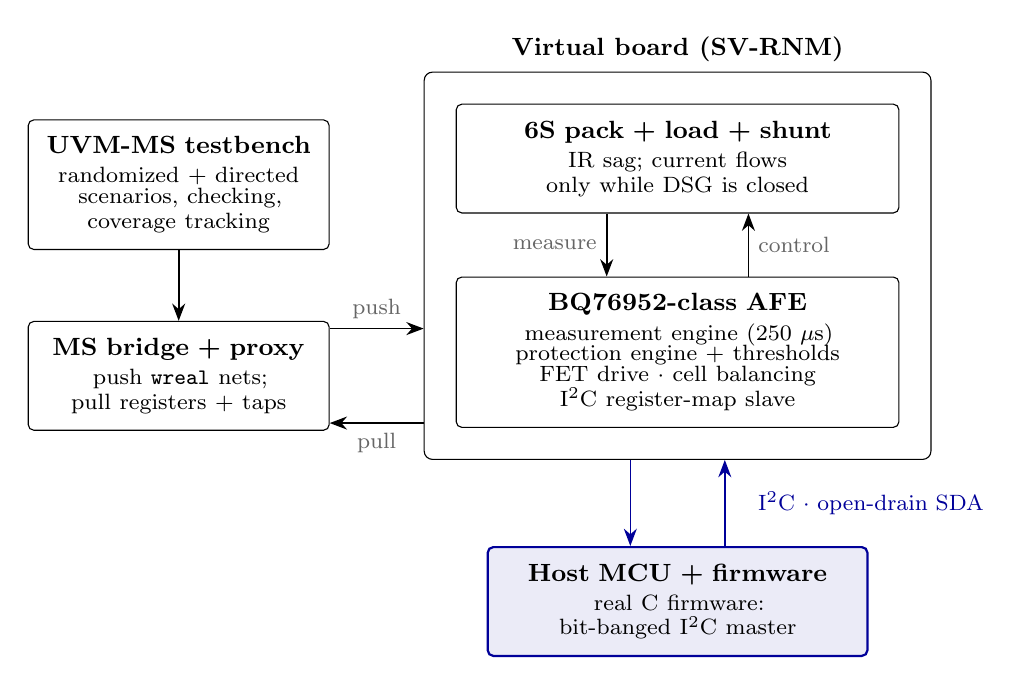
\begin{tikzpicture}[node distance=6mm and 10mm]
  % left column: testbench stack
  \node[blk, text width=34mm] (env)
    {\textbf{UVM-MS testbench}\\[1pt]
     \footnotesize randomized + directed\\[-2pt]
     \footnotesize scenarios, checking,\\[-2pt]
     \footnotesize coverage tracking};
  \node[blk, text width=34mm, below=9mm of env] (brg)
    {\textbf{MS bridge + proxy}\\[1pt]
     \footnotesize push \texttt{wreal} nets;\\[-2pt]
     \footnotesize pull registers + taps};

  % board container
  \node[blk, text width=52mm, right=16mm of env.north east, anchor=north west,
        yshift=2mm] (pack)
    {\textbf{6S pack + load + shunt}\\[1pt]
     \footnotesize IR sag; current flows\\[-2pt]
     \footnotesize only while DSG is closed};
  \node[blk, text width=52mm, below=8mm of pack] (afe)
    {\textbf{BQ76952-class AFE}\\[1pt]
     \footnotesize measurement engine (250 $\mu$s)\\[-2pt]
     \footnotesize protection engine + thresholds\\[-2pt]
     \footnotesize FET drive $\cdot$ cell balancing\\[-2pt]
     \footnotesize \iic{} register-map slave};
  \node[draw, rounded corners=3pt, inner sep=4mm,
        fit={(pack) (afe)},
        label={[font=\small\bfseries]90:Virtual board (SV-RNM)}]
        (board) {};

  % MCU
  \node[hot, text width=44mm, below=15mm of afe] (mcu)
    {\textbf{Host MCU + firmware}\\[1pt]
     \footnotesize real C firmware:\\[-2pt]
     \footnotesize bit-banged \iic{} master};

  % arrows
  \draw[arr] (env) -- (brg);
  \draw[arr] ([yshift= 6mm]brg.east) -- node[lbl, above]{push}
             ([yshift= 6mm]brg.east -| board.west);
  \draw[arr] ([yshift=-6mm]brg.east -| board.west) --
             node[lbl, below]{pull} ([yshift=-6mm]brg.east);
  \draw[arr] ([xshift= 9mm]afe.north) -- node[lbl, right]{control}
             ([xshift= 9mm]pack.south);
  \draw[arr] ([xshift=-9mm]pack.south) -- node[lbl, left]{measure}
             ([xshift=-9mm]afe.north);
  \draw[arrh] ([xshift=-6mm]board.south) --
              ([xshift=-6mm]board.south |- mcu.north);
  \draw[arrh] ([xshift= 6mm]board.south |- mcu.north) --
              ([xshift= 6mm]board.south);
  \node[lbl, blue!60!black, anchor=west]
    at ([xshift=9mm]$(board.south)!.5!(board.south |- mcu.north)$)
    {\iic{} $\cdot$ open-drain SDA};
\end{tikzpicture}
\caption{System architecture.  The firmware's only window into the
analog world is the \iic{} bus (highlighted); the AFE's FET outputs
feed back into the pack model, closing the analog loop.}
\label{fig:arch}
\end{figure}

The five pieces:

\begin{itemize}
  \item \textbf{6S pack + load + shunt} (\texttt{pack\_rnm.sv}):
    per-cell open-circuit voltage, IR sag under load, shunt sense
    voltage.  Crucially, load current flows only while the AFE's
    discharge FET is closed: the protection loop-back.
  \item \textbf{BQ76952-class AFE} (\texttt{bq76952\_rnm.sv}):
    a 250\,$\mu$s measurement loop with gain tolerance and noise, its
    own protection engine (cell under-/overvoltage with hysteresis,
    latched overcurrent, overtemperature), FET drive, cell balancing
    with the sense-line read-droop artifact, and a pin-level \iic{}
    slave over a register map.
  \item \textbf{\iic{} bus}: open-drain SDA resolved in the testbench
    top ($\mathit{sda} = \overline{\mathit{pull}_m \lor
    \mathit{pull}_s}$).  Every threshold, measurement and balancing
    command crosses it as real bus traffic at ${\sim}400$\,kHz.
  \item \textbf{Host firmware} (\texttt{firmware.c}): unmodified C,
    stepped one MCU clock per DPI call: a queue-based bit-banged
    \iic{} master, threshold configuration at start-up, a 2\,ms poll
    loop, a balancing policy with hysteresis, and a fault-recover
    write.  The tick-shim MCU is one of two execution backends for
    the firmware: Section~\ref{sec:cosim} runs the same logic as
    real ARM instructions on an emulated STM32 under mainline QEMU.
  \item \textbf{UVM-MS layer}: bridge + abstract proxy per UVM-MS~1.0
    clauses 4.2.1/4.2.3.  It pushes scenarios onto \texttt{wreal}
    control nets and pulls \emph{both} sides of the bus (the host's
    beliefs via DPI, and the AFE's actual registers via hierarchical
    reference), plus the analog current tap.
\end{itemize}

%=======================================================================
\section{The analog board model}
%=======================================================================

Figure~\ref{fig:schem} shows the electrical circuit being modelled.
The RNM abstraction keeps the behaviours that can change what firmware
sees and drops everything else: each cell is an ideal source $V_{ci}$
behind an internal resistance $R_{\mathrm{int}}$, the load draws a
commanded current $I_{\mathrm{load}}$ through the discharge FET, and
the pack current develops a millivolt-level sense voltage across the
1\,m$\Omega$ shunt.  (How these models were constructed and
cross-validated against SPICE on the board's fabrication schematic is
the subject of a companion paper; here they are simply the board.
The fabrication schematic itself, including the SWD (J3) and UART
console (J4) headers, is reproduced in Appendix~\ref{app:sch}.)

\begin{figure}[htbp]
\centering
\begin{circuitikz}[scale=0.92, transform shape, font=\small]
  % ---- cell stack (left) ----
  \draw (0,9.0) node[circ]{} node[above]{\textbf{B+}}
        (0,9.0) to[battery1, l=$V_{c6}$] (0,7.8)
                to[R, l=$R_{\mathrm{int}}$] (0,6.9) node[circ]{}
        (0,6.9) to[battery1, l=$V_{c5}$] (0,5.7)
                to[R, l=$R_{\mathrm{int}}$] (0,4.8) node[circ]{};
  \node at (0,4.35) {$\vdots$};
  \draw (0,3.9) node[circ]{}
        (0,3.9) to[battery1, l=$V_{c1}$] (0,2.7)
                to[R, l=$R_{\mathrm{int}}$] (0,1.8) node[circ]{}
        (0,1.8) -- (0,0.6) node[circ]{} node[below]{\textbf{B$-$}};

  % ---- load branch (middle) ----
  \draw (0,9.0) -- (3.2,9.0);
  \draw (3.2,9.0) node[nmos, anchor=D, rotate=90, xscale=-1](dsg){};
  \node[above=1mm of dsg] {DSG};
  \draw (dsg.S) -- (5.6,9.0)
        (5.6,9.0) -- (5.6,3.6)
        (5.6,3.6) to[I, l=$I_{\mathrm{load}}$] (5.6,2.3)
        (5.6,2.3) -- (5.6,1.8)
        (5.6,1.8) to[R, l=$R_{\mathrm{sh}}$, a=1\,m$\Omega$] (2.6,1.8)
        (2.6,1.8) -- (0,1.8);

  % ---- AFE box (right) ----
  \draw[rounded corners=3pt] (8.0,1.2) rectangle (11.6,9.4);
  \node[align=center] at (9.8,8.9) {\textbf{BQ76952-class}\\ \textbf{AFE model}};

  % cell-sense taps
  \draw (0,6.9) -- node[lbl, above, pos=.5]{VC5} (8.0,6.9);
  \draw (0,4.8) -- (8.0,4.8);
  \draw (0,3.9) -- node[lbl, above, pos=.5]{VC1} (8.0,3.9);
  \draw (0,9.0) -- (1.4,9.0) (1.4,9.0) |- node[lbl, above, pos=.9]{VC6} (8.0,7.7);
  % shunt sense
  \draw (5.6,1.8) -- (5.6,1.4) -- (7.0,1.4) -- (7.0,2.4)
        -- node[lbl, above]{SRP} (8.0,2.4);
  \draw (2.6,1.8) -- (2.6,1.0) -- (7.4,1.0) -- (7.4,1.7)
        -- node[lbl, above, pos=.9]{SRN} (8.0,1.7);
  % thermistor (kept clear of the load branch at x=5.6)
  \draw (8.0,6.1) to[thR, l_=NTC] (6.6,6.1) -- (6.6,5.5)
        node[ground]{};
  \node[lbl, above right] at (8.0,6.15) {TS};

  % FET gate drive
  \draw[arr] (9.0,9.4) |- node[lbl, above, pos=.8]{gate drive} (dsg.G);

  % I2C to host
  \draw (11.6,4.6) -- node[lbl, above]{SDA} (13.0,4.6);
  \draw (11.6,3.7) -- node[lbl, above]{SCL} (13.0,3.7);
  \node[blk, anchor=west, text width=17mm] at (13.0,4.15)
        {\textbf{Host}\\ \textbf{MCU}};
\end{circuitikz}
\caption{The modelled circuit.  Cells $V_{c1..6}$ with per-cell
$R_{\mathrm{int}}$ feed the load through the AFE-controlled DSG FET;
the pack current develops the sense voltage across
$R_{\mathrm{sh}}$.  The AFE samples the cell taps, shunt pair and NTC,
and the host reaches everything through two \iic{} wires.  (CHG FET
and charger path omitted; out of scope for this version.)}
\label{fig:schem}
\end{figure}

Three modelling choices matter to the verification story:

\begin{description}
  \item[Loop-back is physical.]  $I_{\mathrm{load}}$ flows only while
    DSG is on: $i_{\mathrm{act}} = \mathrm{DSG} \cdot
    I_{\mathrm{load}}$, and every cell terminal sits at
    $V_{ci} - i_{\mathrm{act}} R_{\mathrm{int}}$.  A protection trip
    therefore changes the very measurements the firmware reads next.
  \item[The shunt-sense node is a summing net.]  It is declared with a
    user-defined nettype whose resolution function sums driver
    contributions (UVM-MS 4.2.3.2): the shunt model and a 20\,kHz
    DC/DC ripple interferer share the net, and the \emph{net type},
    not the testbench, decides how they combine.
  \item[Balancing has its measurement artifact.]  A cell being bled
    through its sense line reads ${\sim}40$\,mV low (the well-known
    BQ-family effect), so the scoreboard predicts it rather than
    widening a tolerance.
\end{description}

%=======================================================================
\section{The AFE register map and the \iic{} bus}
%=======================================================================

Table~\ref{tab:regmap} lists the demo register map.  Direct-command
measurement addresses follow the real BQ76952; the real part's RAM
configuration (subcommand 0x3E/0x3F plus checksum at 0x60) is
flattened into directly writable registers, a documented
simplification.

\begin{table}[htbp]
\centering\small
\begin{tabular}{@{}lll@{}}
\toprule
Address & Register & Access \\
\midrule
\reg{0x03}        & Safety Status A: CUV, COV, OCD, OT bits & RO \\
\reg{0x14}+2$n$   & Cell $n{+}1$ voltage, mV, little-endian & RO \\
\reg{0x3A/3B}     & Pack current, mA, signed                & RO \\
\reg{0x68/69}     & Temperature, 0.1\,$^\circ$C, signed     & RO \\
\reg{0x7F}        & FET status: DSG, CHG bits               & RO \\
\reg{0x90/91}     & CUV threshold, mV                       & RW \\
\reg{0x92/93}     & COV threshold, mV                       & RW \\
\reg{0x94/95}     & OCD threshold, mA                       & RW \\
\reg{0x96}        & Protection enable bits                  & RW \\
\reg{0x97}        & FET allow: DSG, CHG                     & RW \\
\reg{0x98}        & Cell-balancing active mask              & RW \\
\reg{0x99}        & Recover: write 1 clears latched OCD     & W  \\
\bottomrule
\end{tabular}
\caption{Demo register map of the AFE model (BQ76952-flavoured).}
\label{tab:regmap}
\end{table}

The slave is modelled at pin level: START/STOP detection on SDA edges
gated by SCL, bit assembly on SCL rising edges, ACK generation, a
register pointer with burst auto-increment, and write protection on
the read-only ranges.  Figure~\ref{fig:i2c} shows the start of a
threshold-write transaction, and the one-clock-edge subtlety that
produced the first bring-up bug.

\begin{figure}[htbp]
\centering
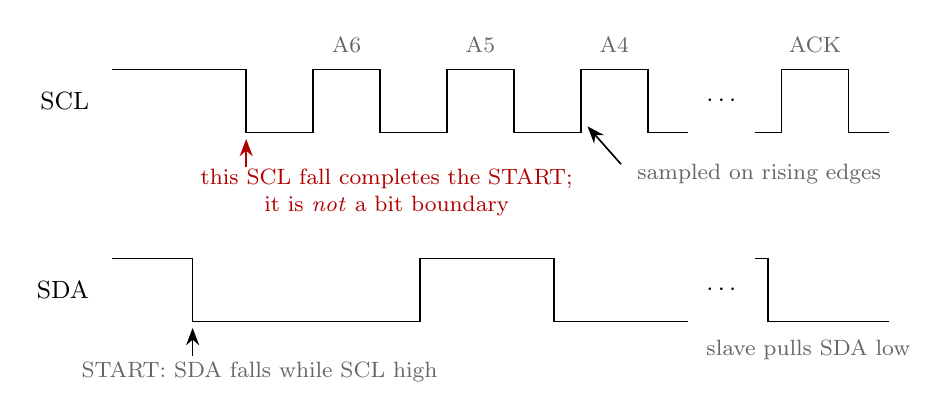
\begin{tikzpicture}[x=8.5mm, y=8mm, font=\small]
  % ---- SCL (high = 5, low = 4) ----
  \node[left] at (-0.2,4.5) {SCL};
  \draw[semithick]
    (0,5) -- (2.0,5)
    -- (2.0,4) -- (3.0,4)
    -- (3.0,5) -- (4.0,5) -- (4.0,4) -- (5.0,4)
    -- (5.0,5) -- (6.0,5) -- (6.0,4) -- (7.0,4)
    -- (7.0,5) -- (8.0,5) -- (8.0,4) -- (8.6,4);
  \node at (9.1,4.5) {$\cdots$};
  \draw[semithick]
    (9.6,4) -- (10.0,4) -- (10.0,5) -- (11.0,5) -- (11.0,4) -- (11.6,4);

  % ---- SDA (high = 2, low = 1) ----
  \node[left] at (-0.2,1.5) {SDA};
  \draw[semithick]
    (0,2) -- (1.2,2)
    -- (1.2,1) -- (4.6,1)
    -- (4.6,2) -- (6.6,2)
    -- (6.6,1) -- (8.6,1);
  \node at (9.1,1.5) {$\cdots$};
  \draw[semithick] (9.6,2) -- (9.8,2) -- (9.8,1) -- (11.6,1);

  % bit labels above SCL
  \node[lbl] at (3.5,5.4) {A6};
  \node[lbl] at (5.5,5.4) {A5};
  \node[lbl] at (7.5,5.4) {A4};
  \node[lbl] at (10.5,5.4) {ACK};

  % START annotation, below SDA
  \draw[arr] (1.2,0.45) -- (1.2,0.9);
  \node[lbl] at (2.2,0.2) {START: SDA falls while SCL high};

  % the bug annotation, in the band between the rails
  \draw[arr, red!70!black] (2.0,3.45) -- (2.0,3.9);
  \node[lbl, red!70!black, align=center] at (4.1,3.05)
    {this SCL fall completes the START;\\
     it is \emph{not} a bit boundary};

  % sampling convention, right side of the band
  \draw[arr] (7.6,3.5) -- (7.1,4.1);
  \node[lbl, anchor=west] at (7.7,3.35) {sampled on rising edges};

  % ACK note, below SDA at the right
  \node[lbl] at (10.4,0.55) {slave pulls SDA low};
\end{tikzpicture}
\caption{Start of an \iic{} transaction (address byte
\reg{0x10} = device 0x08, write).  The v1 slave model counted the SCL
falling edge that completes the START condition as a data-bit
boundary, assembled every address one bit short, and NACKed every
transaction: the host read 0xFF everywhere.  The fix: only a
falling edge that ends a real clock pulse advances the bit counter.}
\label{fig:i2c}
\end{figure}

%=======================================================================
\section{The UVM-MS layer: closing three loops}
%=======================================================================

The verification value comes from three loops that each cross the
firmware/analog boundary in both directions
(Figure~\ref{fig:loop}).

\begin{figure}[htbp]
\centering
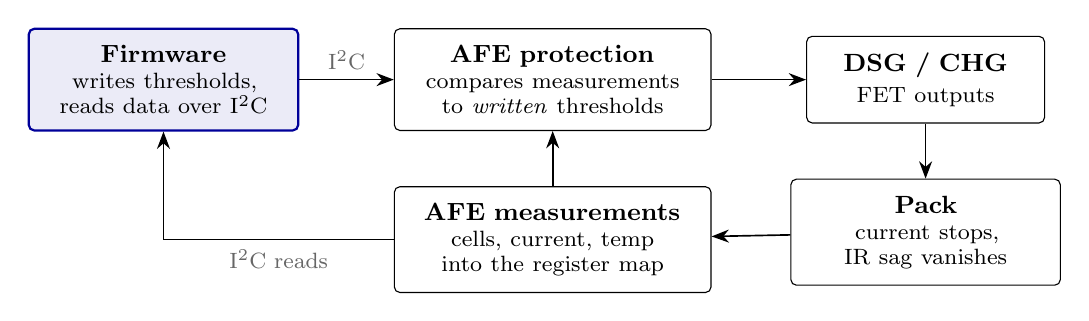
\begin{tikzpicture}[font=\small, node distance=7mm and 12mm]
  \node[hot, text width=30mm] (fw)  {\textbf{Firmware}\\
        \footnotesize writes thresholds,\\[-2pt]
        \footnotesize reads data over \iic{}};
  \node[blk, text width=36mm, right=of fw] (prot) {\textbf{AFE protection}\\
        \footnotesize compares measurements\\[-2pt]
        \footnotesize to \emph{written} thresholds};
  \node[blk, text width=26mm, right=of prot] (fet) {\textbf{DSG / CHG}\\
        \footnotesize FET outputs};
  \node[blk, text width=30mm, below=of fet] (pack) {\textbf{Pack}\\
        \footnotesize current stops,\\[-2pt]
        \footnotesize IR sag vanishes};
  \node[blk, text width=36mm, below=of prot] (meas) {\textbf{AFE measurements}\\
        \footnotesize cells, current, temp\\[-2pt]
        \footnotesize into the register map};

  \draw[arr] (fw) -- node[lbl, above]{\iic{}} (prot);
  \draw[arr] (prot) -- (fet);
  \draw[arr] (fet) -- (pack);
  \draw[arr] (pack) -- (meas);
  \draw[arr] (meas) -- (prot);
  \draw[arr] (meas) -| node[lbl, below, pos=.25]{\iic{} reads} (fw);
\end{tikzpicture}
\caption{The closed verification loop: a protection decision changes
the analog state, which changes the next measurements, which the
firmware reads back over the same bus it configured the protection
through.}
\label{fig:loop}
\end{figure}

\begin{enumerate}
  \item \textbf{Configuration integrity.}  The host writes CUV
    2800\,mV, COV 4250\,mV, OCD 3000\,mA at start-up.  The scoreboard
    does not trust the write: it reads the AFE's threshold registers
    directly and fails any scenario where the values the protection
    engine actually uses differ from the host's intent.  A byte-order
    bug, a wrong register address, or a broken bus all fail here.
  \item \textbf{Protection loop-back.}  When the AFE trips, the
    scoreboard checks the \emph{analog} consequence (shunt current
    exactly 0\,mA), not just the status bit, plus a trip-latency
    bound of three host control loops.
  \item \textbf{Balancing closed-loop.}  When the cell spread exceeds
    50\,mV, the host must write the balancing mask for exactly the
    highest cell; the scoreboard checks the AFE register, and that the
    cell's reading droops the predicted 40\,mV.
\end{enumerate}

Prediction is white-box and two-pass: first compute what the AFE will
measure assuming the discharge path is closed
($V_{ci} - I_{\mathrm{load}}R_{\mathrm{int}}$ scaled by gain
tolerance; current scaled and offset), decide from those values which
protections must trip, then recompute the final measurements with the
resulting current.  Checks are skipped only in narrow bands around
each threshold, where noise legitimately makes the outcome go either
way.

%=======================================================================
\section{Results}
%=======================================================================

The regression (seed~1) runs 13 scenarios in ${\sim}291$\,ms of
simulated time and passes with zero failures
(Table~\ref{tab:results}).

\begin{table}[htbp]
\centering\small
\begin{tabular}{@{}p{34mm}p{44mm}p{62mm}@{}}
\toprule
Scenario & Setup & Observed \\
\midrule
Safe corners (4, random) & cells 3.29--3.66\,V, load $\le$1.2\,A,
  16--47\,$^\circ$C, tolerances randomized &
  readings match prediction to ${\sim}1$\,mV per cell and tens of mA;
  both FETs closed \\
Cell undervoltage & all cells 2.65\,V &
  status 0x1; DSG opens; current stops; cells read unloaded \\
Cell overvoltage & all cells 4.32\,V &
  status 0x2; CHG opens; DSG stays closed \\
Overcurrent & 4.2\,A load &
  status 0x4; trip in 0 host loops, latched; shunt current 0\,mA \\
Overtemperature & 70\,$^\circ$C &
  status 0x8; both FETs open \\
Imbalance & cell~4 at $+90$\,mV &
  host writes CB mask 0x8; AFE register confirms; cell~4 droops the
  predicted 40\,mV \\
DC/DC ripple & 20\,kHz interferer on the shunt net &
  current wobbles inside the widened tolerance; no false trip \\
Hero (3 phases) & 1\,A $\to$ 4.2\,A (no reset) $\to$ 1\,A (host reset) &
  normal $\to$ OCD latches, current physically stops $\to$ recover
  write over \iic{} restores 1\,A operation \\
\bottomrule
\end{tabular}
\caption{The 13-scenario regression, seed 1.  Functional coverage
crosses physical corner against firmware response (load band $\times$
DSG, voltage band $\times$ CHG, imbalance $\times$ balancing).}
\label{tab:results}
\end{table}

\subsection*{The bench caught its own bring-up bugs}

The strongest evidence that the checks have teeth: three real defects
surfaced before the first passing run, each found by a specific check.

\begin{enumerate}
  \item \textbf{The START-edge protocol bug}
    (Figure~\ref{fig:i2c}): every host read returned 0xFF; found by
    the configuration-integrity check (``thresholds never arrived'').
  \item \textbf{Empty array arguments}: cell voltages pushed through
    an unpacked-array argument on the virtual proxy method arrived
    empty (a simulator edge case), so the AFE measured 0\,V and its
    own undervoltage protection latched the pack off; found by the
    loop-back check.  The push path now uses scalars throughout.
  \item \textbf{A units error} (A vs.\ mA) in the AFE current path
    made every current reading $1000\times$ low; found by the
    current-accuracy check on the very first smoke run.
\end{enumerate}

%=======================================================================
\section{Real firmware on an emulated SoC: QEMU co-simulation}
\label{sec:cosim}
%=======================================================================

A firmware team's test ladder has three rungs: host-compiled unit
tests of the logic (fast, run on every commit), the real binary on an
emulator or virtual platform (pre-silicon, in CI), and real silicon
on a bench or HIL rig.  This demonstrator climbs the first two,
and upgrades both, because on either rung the thing on the other side
of the firmware is normally a \emph{mock}, and here it is the SV-RNM
board.  Everything before this section is rung one: the decision
logic, host-compiled and stepped through DPI, graded by the
testbench across randomized scenarios against the board's physics
instead of against stubs.  This section is rung two, with no shim
at all.

The distinction is concrete: the two rungs compile the \emph{same}
firmware source with two different compilers, for two different
universes.  On rung one, the \emph{host} compiler (plain
\texttt{gcc}, targeting the x86-64 machine the simulator itself runs
on) builds the logic into a native shared library that xezim
loads through DPI; the testbench calls \texttt{fw\_tick()} once per
modelled MCU clock and the host CPU executes the decision logic
directly.  That is what makes rung one cheap and transparent:
fast enough to run randomized scenarios by the hundred, and open
enough that the testbench can predict and check every reading the
firmware takes.  But it also means the firmware
lives in the host's universe: the operating system's loader performs
startup, integer widths and alignment come from x86-64, and there is
no memory map at all, so an entire class of defects (startup code,
vector table, linker layout, register-level driver access,
cross-compiler surprises) cannot even be expressed, let alone
caught.  On rung two, the cross-compiler
(\texttt{arm-none-eabi-gcc}) builds the same source into an ARM
Thumb bare-metal ELF that the emulated Cortex-M boots from its reset
vector, instruction by instruction, registers and all.  Each rung
exists to catch its bug class at the cheapest level that can express
it: rung one finds logic bugs by the thousand; rung two proves the
shippable artifact (the binary that would be flashed) holds
the same conversation with the same board.

QEMU is the emulator custom-SoC teams typically build their
pre-silicon firmware flows on, extending it with machine and device
models of their own silicon.  So the same host logic, written as
\emph{natural} blocking C (the queue-based \iic{} state machine
dissolves under an emulator) and compiled to a ${\sim}4$\,kB
bare-metal ELF, runs as real ARM instructions on \emph{unmodified
mainline} QEMU (9.2.4, machine \texttt{netduinoplus2}, an STM32F405
Cortex-M4) and drives the SV-RNM board in xezim through a lockstep
TCP bridge (Figure~\ref{fig:cosim}).

Mainline QEMU has no generic remote-MMIO hook, so the bridge rides a
spare UART: \mbox{USART1}'s character device is a TCP socket into
the xezim bridge server, and the firmware speaks a three-command
line protocol (\texttt{S}~set pins, \texttt{A}~advance board time,
\texttt{F}~finish, each acknowledged with the settled SDA) through
the UART's data register, the bolt-onto-a-spare-port pattern such
teams use for HIL and model channels.  The schematic's U2 is an
STM32G0B1, a part mainline QEMU does not model; the mission firmware
is core-agnostic behind a five-function platform HAL
(\texttt{hal.h}), and a G0B1 machine model is precisely the kind of
extension a tapeout team would add to its QEMU fork: for custom
silicon, the machine model \emph{is} part of the deliverable.

\begin{figure}[htbp]
\centering
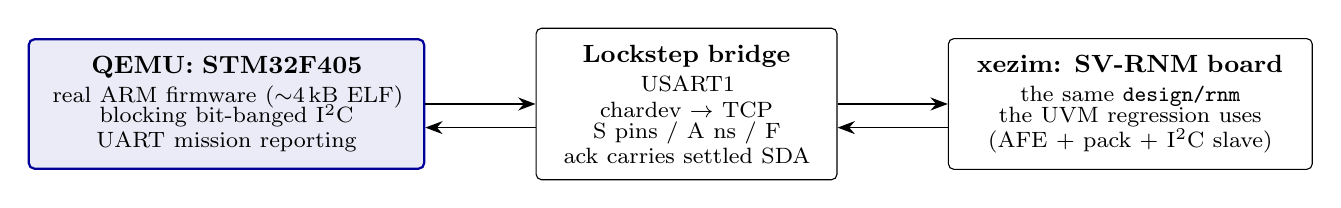
\begin{tikzpicture}[node distance=6mm and 14mm]
  \node[hot, text width=46mm] (rn)
    {\textbf{QEMU: STM32F405}\\[1pt]
     \footnotesize real ARM firmware (${\sim}4$\,kB ELF)\\[-2pt]
     \footnotesize blocking bit-banged \iic{}\\[-2pt]
     \footnotesize UART mission reporting};
  \node[blk, text width=34mm, right=of rn] (br)
    {\textbf{Lockstep bridge}\\[1pt]
     \footnotesize USART1 chardev $\to$ TCP\\[-2pt]
     \footnotesize S pins / A ns / F\\[-2pt]
     \footnotesize ack carries settled SDA};
  \node[blk, text width=42mm, right=of br] (xz)
    {\textbf{xezim: SV-RNM board}\\[1pt]
     \footnotesize the same \texttt{design/rnm}\\[-2pt]
     \footnotesize the UVM regression uses\\[-2pt]
     \footnotesize (AFE + pack + \iic{} slave)};
  \draw[arr] (rn) -- (br);
  \draw[arr] (br) -- (xz);
  \draw[arr] ([yshift=-3mm]xz.west) -- ([yshift=-3mm]br.east);
  \draw[arr] ([yshift=-3mm]br.west) -- ([yshift=-3mm]rn.east);
\end{tikzpicture}
\caption{Co-simulation topology.  Board time advances \emph{only} on
the firmware's own delay commands, so bit-banged \iic{} is
cycle-honest and the board timeline is reproducible.}
\label{fig:cosim}
\end{figure}

The synchronization contract does the heavy lifting: the board's
clock moves only when the firmware spends time (an \texttt{A}
command), and every pin update is acknowledged with the freshly
settled SDA.  QEMU's own host-side scheduling is not deterministic,
but the board timeline is: consecutive runs end at
$t = 52{,}233{,}121$\,ns exactly, with identical mission logs,
because the contract makes board time a function of the firmware's
stated delays alone, not of host timing, instruction counts, or
the core executing them.  A full mission takes ${\sim}8$\,s of wall
clock.  One practical note from bring-up: the command/ack
round-trips are tiny TCP packets, so Nagle's algorithm must be off
on both ends (\texttt{nodelay=on} on QEMU's chardev); with it on,
the identical run takes minutes instead of seconds.

The mission (configure protection over \iic{}, ride out an
overload the \emph{AFE in the RNM} trips, recover the latch) in
the firmware's own UART log:

{\small
\begin{verbatim}
[fw] BMS host up on QEMU/STM32F405; board = SV-RNM in xezim
[fw t=1.9ms]  AFE protection configured (CUV 2800mV COV 4250mV OCD 3000mA)
[fw t=5.3ms]  ss=0x0 c1=3688mV i=998mA
[fw t=15.2ms] ss=0x0 c1=3688mV i=1004mA
[fw t=18.6ms] ss=0x4 c1=3701mV i=1mA
[fw t=18.6ms] *** OCD TRIP seen over I2C -- current stopped by the AFE
[fw t=48.9ms] recover written (0x99=1)
[fw t=52.2ms] ss=0x0 c1=3694mV i=499mA
[fw t=52.2ms] *** RECOVERED: latch cleared, current flowing again (499mA)
\end{verbatim}
}

Every number is physically consistent with every other domain:
3688\,mV is the 1\,A IR sag, 3701\,mV the unloaded recovery the trip
causes, and 3694\,mV is exactly $3700 - 0.5\,\mathrm{A} \times
12\,\mathrm{m}\Omega$ after recovery at the reduced load.  The AFE
tripped 250\,$\mu$s (one measurement cycle) after the overload,
observed from the board side in the xezim log and from the chip side
over \iic{}, through a bus whose every edge was produced by ARM
instructions.

\subsection{Fault injection: does the framework actually catch bugs?}
\label{sec:faults}

A verification environment earns trust by catching defects it was not
tuned for, so the co-simulation's pass criterion is not a log grep
but a \emph{cross-domain checker} (\texttt{check\_cosim.py}): it
treats the firmware's UART log and the board's xezim log as two
independent witnesses and cross-examines them under four rules, one
per layer of the stack: R1, a real overload must open DSG within
2\,ms; R2, chip-reported telemetry must match board physics during
the quiet phase (3688$\pm$5\,mV, 1000$\pm$15\,mA); R3, DSG must never
open \emph{before} an overload exists; R4, bus and mission health (no
NACKs, no implausible readings, trip-and-recover must complete).  The
firmware itself carries defence-in-depth: NACK counting and a
plausibility window on cell voltage, both reported on its UART.

A campaign (\texttt{run\_faults.sh}) then injected one deliberate
defect into each layer.  Every fault was caught, each by a
\emph{different} rule, while the clean setup stayed green:

\begin{table}[htbp]
\centering
\small
\begin{tabular}{@{}llll@{}}
\toprule
Run & Layer & Injected defect & Caught by \\
\midrule
clean     & n/a       & none                              & passes (trip $+0.25$\,ms) \\
fw\_cfg   & FW config & OCD threshold write byte-swapped  & R1: ``overload at 15\,ms \\
          &           & (3000\,mA arms as 47\,115\,mA)    & \quad but DSG opened \emph{never}'' \\
fw\_proto & FW protocol & cell readout off by one register & R2: ``c1=26894\,mV; board \\
          &           &                                   & \quad truth is 3688$\pm$5'' \\
board     & analog RNM & $+2500$\,mA current-path offset  & R3: ``DSG opened at 1.25\,ms, \\
          &           & (damaged sense front-end)         & \quad \emph{before} the overload'' \\
bridge    & pin path  & SDA readback stuck at 1           & R4: slave not ACKing + \\
          &           & (pin-mux class of bug)            & \quad implausible telemetry \\
\bottomrule
\end{tabular}
\caption{Fault-injection campaign: one defect per layer, each caught
by its own rule.  Evidence per run in
\texttt{logs\_qemu/faults/}.}
\label{tab:faults}
\end{table}

The analog fault produces the campaign's best exhibit.  With a
$+2.5$\,A offset in the current path, the firmware reads
\texttt{c1=3700mV i=2498mA}: current ``flowing'' alongside \emph{zero}
IR sag, a physically impossible pair: precisely how a bench
engineer would recognise a sense-path offset.  Its recovery attempts
fail forever, because the AFE instantly re-trips on the phantom
current.  A real analog front-end defect, diagnosed purely from the
chip's own telemetry, before any hardware exists: the class of
board-bring-up mystery this framework was built to catch.  The
byte-swap fault makes the complementary point: the system behaves
\emph{perfectly} at 1\,A and betrays nothing until the day of the
first real overload, which is why R1 watches the board's truth rather
than the firmware's belief.

%=======================================================================
\section{Limitations and next steps}
%=======================================================================

Deliberate simplifications, each with a clear upgrade path:

\begin{itemize}
  \item \textbf{Register map.}  The subcommand-plus-checksum RAM
    configuration protocol of the real part is flattened into direct
    registers; temperature is reported in 0.1\,$^\circ$C rather than
    0.1\,K.
  \item \textbf{Uneven rung coverage.}  Rung one (host-compiled
    logic through DPI) carries the 13-scenario randomized
    suite; rung two (the ARM binary under QEMU,
    Section~\ref{sec:cosim}) runs one directed mission.  Pointing
    the testbench's stimulus at the bridge is the natural
    unification.  (A randomized campaign per emulated-firmware run
    would also be slow; rung one remains the regression workhorse.)
    And the emulated part is an STM32F405 standing in for the
    schematic's STM32G0B1; a G0B1 machine model in a QEMU fork closes
    that gap.
  \item \textbf{Scope.}  Charge-side current, coulomb counting,
    \iic{} clock stretching and multi-master, and CAN are out of
    scope for this version.
\end{itemize}

Because the bus is modelled at pin level, bus fault injection is a
cheap extension.
Section~\ref{sec:faults} opened that front with a stuck SDA readback,
and the rest of the menu (NACK storms from the slave side, corrupted
bytes, a held SCL) remains the natural next test dimension: does the
host firmware fail safe when its only window into the analog world
degrades?

This demonstrator is the fourth in a series built on one architecture
(RNM board / \texttt{wreal} scenario nets / MS bridge with an
Annex-A proxy / DPI-tick firmware): a TCD1304 CCD sensor channel, an
HX717 load-cell chain, an STM32 internal-ADC BMS, and this one,
each adding one integration step, ending here with a configurable
smart AFE behind a real bus.

%=======================================================================
\appendix
\section{The board schematic}
\label{app:sch}
%=======================================================================

Figure~\ref{fig:fabsch} reproduces the board's fabrication schematic
(KiCad export).  Landmarks for this paper: U2 is the STM32G0B1 host
MCU, U1 the battery-monitor AFE, RS1 the 1\,m$\Omega$ shunt, J1 the
six-cell pack connector, J2 the load, J3 the SWD programming header,
and J4 the UART console header carrying USART2 (PA2/PA3), the serial
port whose log Section~\ref{sec:cosim} captures.  Construction and
cross-tool validation of the sheet are covered in the companion
paper.

\begin{figure}[p]
\centering
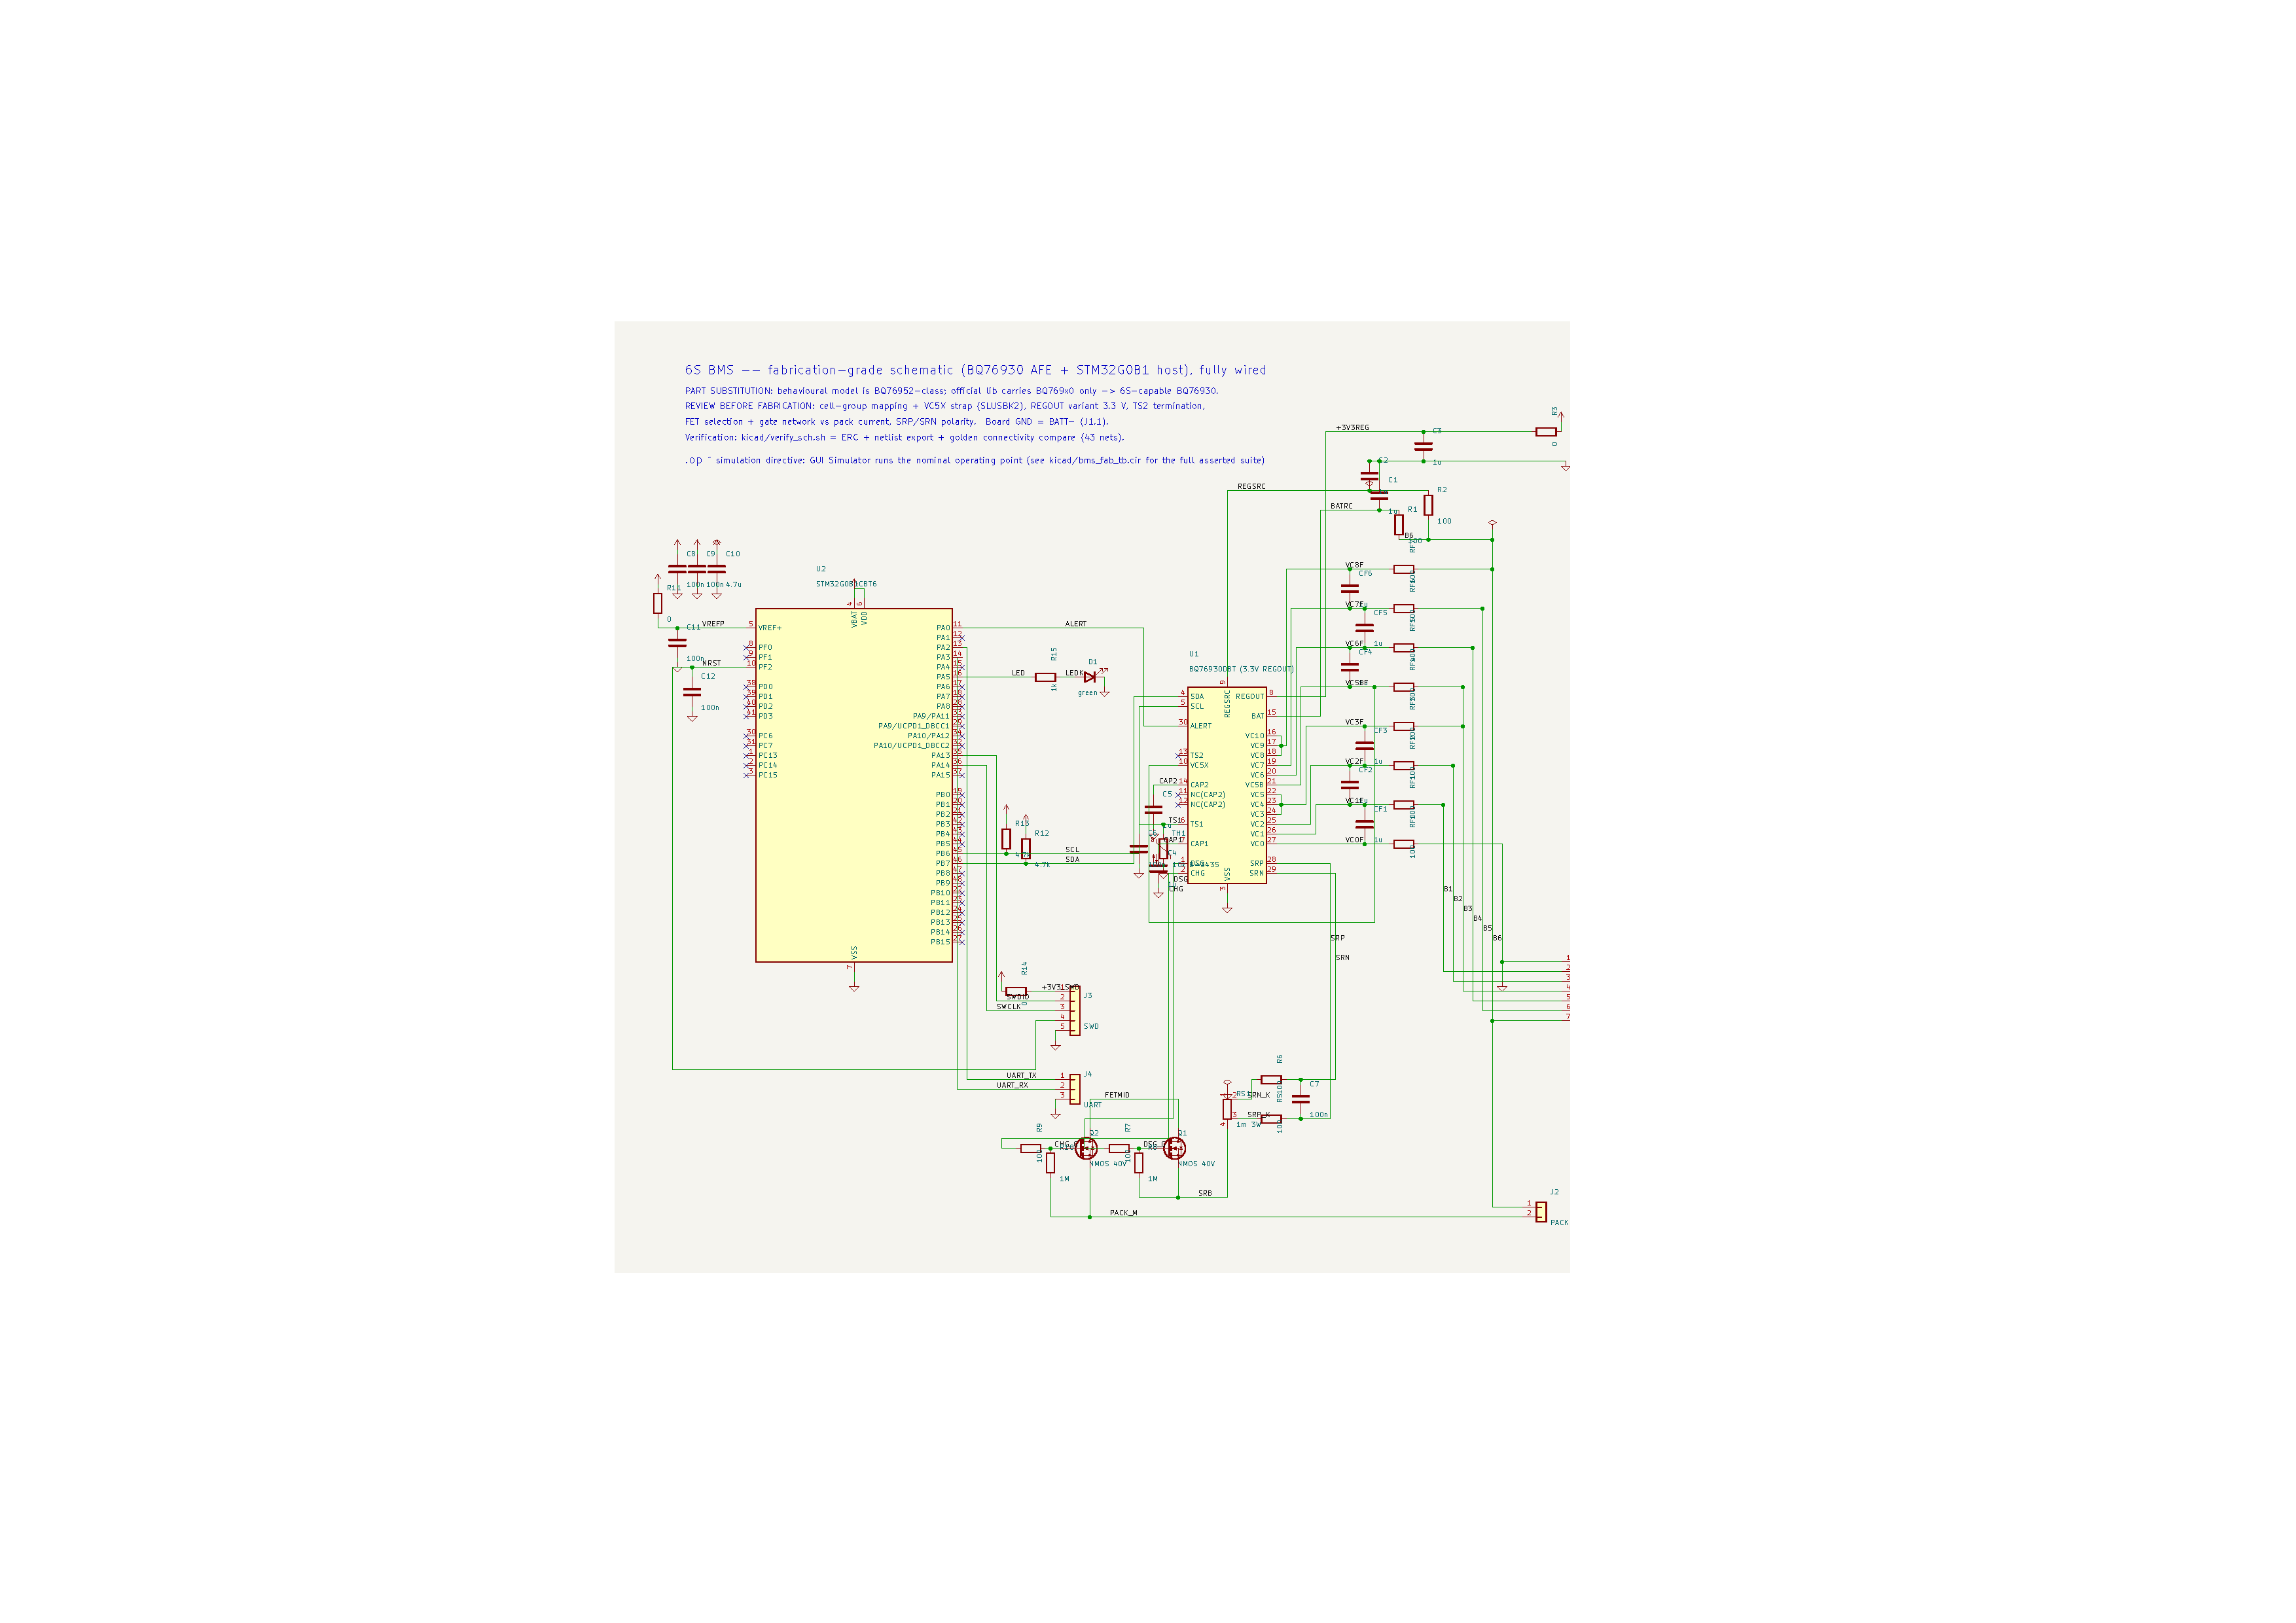
\includegraphics[width=\textwidth, height=0.92\textheight,
                 keepaspectratio]{board_schematic.pdf}
\caption{The 6S BMS fabrication schematic, cropped to the drawn
content.  The UART console header J4 sits below the SWD header J3,
left of the FET cluster.}
\label{fig:fabsch}
\end{figure}

\end{document}
